\section{System Model and Problem Formulation}

\subsection{Network Architecture}

We consider a two-tier V2X network comprising N vehicles, R roadside units (RSUs) each co-located with a MEC server, and a base station (BS) providing wide-area LTE and 5G-NR coverage. Each vehicle has an on-board ECU capable of 2-5 Tera Operations Per Second (TOPS) and a multi-RAT module supporting LTE, ITS-G5, WiFi-6, and 5G-NR simultaneously. \Cref{fig:network_topology} illustrates the system architecture.

\begin{figure}[htbp]
\centering
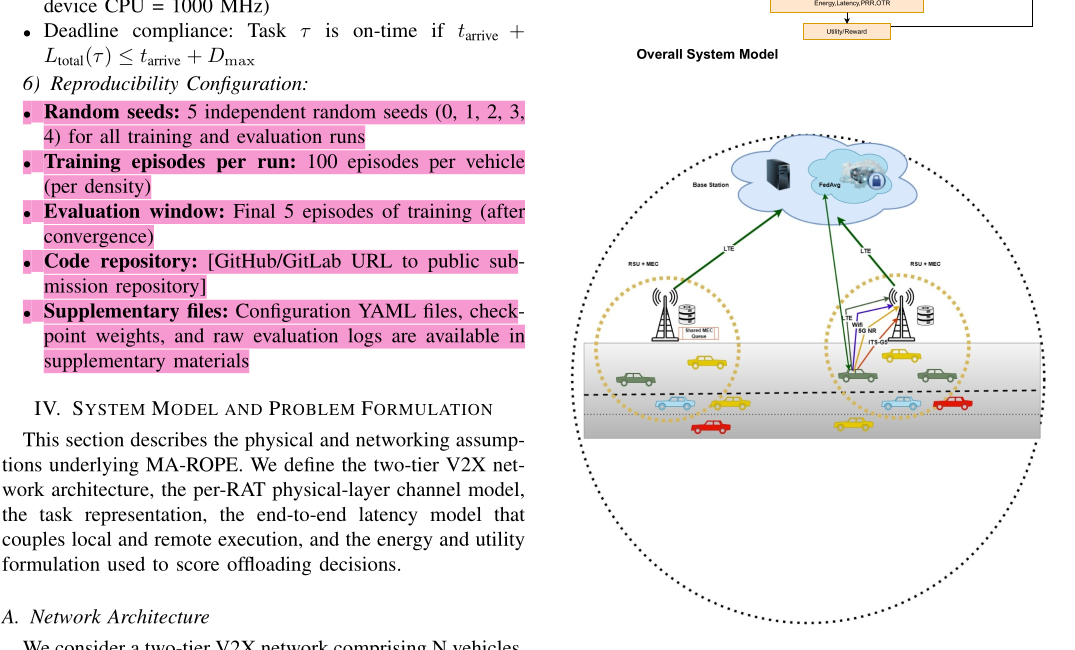
\includegraphics[width=\linewidth,keepaspectratio]{figures/real_fig2b.png}
\caption{Network Topology with 4-RAT heterogeneous access and FedAvg coordination.}
\label{fig:network_topology}
\end{figure}

\subsection{RAT Physical Layer Model}

Following Yacheur et al. \cite{yacheur2023} \Cref{tab:rat_physical}, we assign per-RAT physical parameters as in \Cref{tab:rat_physical}. LTE and 5G-NR operate at -110 dBm noise floor; ITS-G5 and WiFi-6 at -90 dBm. Cellular RATs experience Jakes Doppler fading at vehicular speeds; ITS-G5 and WiFi-6 use the Constant Speed propagation model, as analyzed in Fig. 14.

\begin{table}[h!]
\caption{RAT Physical Parameters (Yacheur 2023 + 3GPP Standards)}
\label{tab:rat_physical}
\centering
\resizebox{\columnwidth}{!}{%
\begin{tabular}{|l|c|c|c|c|c|c|}
\hline
\textbf{RAT} & \textbf{Delay} & \textbf{Throughput} & \textbf{Noise Floor} & \textbf{Fading} & \textbf{Path Loss} & \textbf{Source} \\
\hline
LTE & 20 ms & 50 Mbps & -110 dBm & Jakes & TR 36.885 & \cite{yacheur2023} \\
ITS-G5 & 10 ms & 27 Mbps & -90 dBm & Constant & TR 36.885 & \cite{yacheur2023} \\
WiFi-6 & 5 ms & 600 Mbps & -90 dBm & Constant & 802.11ax & \cite{ieee80211ax} \\
5G-NR & 1 ms & 1 Gbps & -110 dBm & Jakes & TR 38.901 & \cite{3gpp2022} \\
\hline
\end{tabular}%
}
\end{table}


The Signal-to-Interference-plus-Noise Ratio (SINR) for RAT $r$ at distance $d$ with vehicle speed $v$ governs per-PDU delivery probability:

\begin{equation}
\label{eq:sinr}
\text{SINR}_r(d,v) = P_{tx} - \text{PL}_r(d) - N_r - Sh_r - F_r(v)
\end{equation}

where $\text{PL}_r(d)$ is RAT-specific path loss, $N_r$ is noise floor, $Sh_r \sim \mathcal{N}(0,\sigma^2_r)$ is shadowing, and $F_r(v)$ is Jakes fading loss. SINR drives a per-PDU Bernoulli draw with $p_{link} = \sigma(\text{SINR}_r - \theta_r)$ but is NOT the reported PRR metric. Packet Reception Ratio is defined empirically from actual packet counters:

\begin{equation}
\label{eq:prr}
\text{PRR} = \frac{n_{rx}}{n_{tx}}
\end{equation}

where $n_{tx}$ is the number of offload PDU transmission attempts and $n_{rx}$ is PDUs successfully delivered. This separates the physical link model from the reported metric: PRR reflects real packet outcomes, not a smoothed SINR function. Per-RAT empirical PRR fills observation slots obs[4:8]; slots default to 0.5 (unknown) before any attempt on that RAT. The raw link delivery probability $p_{link}$ is separately tracked in infos["link\_delivery\_prob"] for comparing the physical-layer (PHY) curve against measured PRR.

\subsection{Task Model}

Each vehicle generates task $\tau_i = (C_i, V_i, D_i, T_i)$ where $C_i$ is computational workload (CPU cycles), $V_i$ is data volume (MB), $D_i$ is the task's deadline, its maximum tolerable delay (ms), and $T_i \in \{\text{safety}, \text{infotainment}, \text{compute}\}$ determines that deadline: safety tasks require $D_i = 100$ ms (e.g., 3GPP TR 36.885~\cite{molina2017}), infotainment 500 ms, compute 2000 ms.

\subsection{End-to-End Latency Model}

End-to-end task latency is the primary measurable QoS quantity in this work. For each offload PDU attempt at step t, the total latency decomposes into six additive components:

\begin{subequations}
\label{eq:latency_all}
\begin{equation}
\label{eq:ltotal_base}
L_{total} = L_{prop} + L_{tx} + L_{queue} + L_{remote} + L_{rx} + L_{prop}
\end{equation}

where $L_{prop} = d/(2c/3)$ is propagation delay over vehicle-to-RSU distance d at 2/3 speed of light; $L_{tx} = V_i/\text{BW}_r$ is uplink transmission delay for data volume $V_i$ (MB) over RAT bandwidth $\text{BW}_r$; $L_{remote} = C_i/f_{MEC}$ is remote compute delay for workload $C_i$ (CPU cycles) at MEC frequency $f_{MEC}$; $L_{rx}$ is the downlink reception delay for the computed results; and $L_{queue} = 1/(\mu_k - \lambda_k)$ is the M/M/1 queuing delay at the shared RSU, where $\mu_k$ is the server service rate and $\lambda_k$ is the total vehicle arrival rate across all co-located vehicles. The $L_{queue}$ term is the critical shared-resource term: it couples all vehicles' decisions through the common RSU queue and is responsible for the AllOffload collapse observed in Section V.

For partial offloading with ratio $\rho$, local and remote execution proceed in parallel following the model of Mao et al. \cite{mao2017}. The realized end-to-end delay is:

\begin{equation}
\label{eq:ltotal_partial}
\begin{split}
L_{total} =& L_{prop} + \rho \cdot L_{tx} \\
&+ \max(\rho \cdot L_{remote} + L_{rx} + L_{prop}, (1-\rho) \cdot L_{local}) \\
&+ L_{queue}
\end{split}
\end{equation}

where $\rho \in \{0.25, 0.50, 0.75, 1.0\}$ is the partial offload ratio, $\rho \cdot L_{tx}$ captures the transmitted data fraction, and $L_{local} = C_i/f_{ECU}$ is local ECU compute time. When $\rho = 0$ (pure local execution), $L_{total} = L_{local}$ and no PDU is transmitted over the radio; such steps are excluded from latency QoS accounting since no V2X packet is at risk.

\textbf{Deadline classification.} Each offload Protocol Data Unit (PDU) outcome is classified into one of three measurable QoS categories relative to the task-type deadline $D_i$: (1) \textit{delivered\_on\_time}, link success and $L_{total} \leq D_i$, a useful delivery; (2) \textit{delivered\_late}, link success and $L_{total} > D_i$, received but stale, so the transmission was wasted; (3) \textit{not\_delivered}, a link failure from the Bernoulli draw on $p_{link}$, i.e. channel loss. The on-time delivery rate is:

\begin{equation}
\label{eq:otr}
\text{OTR} = \frac{n_{rx\_on\_time}}{n_{tx}}
\end{equation}
\end{subequations}

Note that $\text{OTR} \leq \text{PRR}$ always, since PRR counts all link-successful receptions regardless of deadline. The gap ($\text{PRR} - \text{OTR}$) is the latency-induced deadline violation rate: packets the channel delivered but that arrived too late for the application to use. This is the quantity MA-ROPE directly minimises via the $\exp(-L/D)$ term in the utility reward (\Cref{eq:utility_all}).

\subsection{Energy and Utility}

Total energy consumption is modeled as $E_{total} = P_{tx} \cdot L_{tx} + \epsilon_r \cdot \rho \cdot V_i$, where $P_{tx} \cdot L_{tx}$ captures radio transmit energy over the realized transmission duration and $\epsilon_r$ (J/MB) is the RAT-specific processing or transfer energy cost. The implementation used to produce the results in this paper does not evaluate this formula directly; it instead computes energy through a simplified expression that can return negative values for common cases, which we determined makes any energy figure derived from it scientifically unreliable. Absolute energy is therefore not reported anywhere in Section V. The energy term does, however, still enter the $\exp(-E/3)$ component of both utility functions below via that same simplified expression, so the $U_{PRR}$ and $U_{OTR}$ values reported in Section V (Table 6 and the density-scaling results) inherit its unreliability and should be read as reward-shaping and secondary evaluation signals rather than independently validated quantities. This paper's primary claims rest on Fleet OTR, PRR, and the Deadline Retention Ratio, which are computed directly from transmission and deadline outcomes and do not depend on the utility formula or its energy term; see the Discussion and Conclusion for the full disclosure and the path to a validated energy model. MA-ROPE defines two complementary utility functions, each optimized for a different deployment criterion (Yacheur et al. \cite{yacheur2023} Eq. (2) extended):

\begin{subequations}
\label{eq:utility_all}
\begin{equation}
U_{PRR} = \alpha \cdot \text{PRR} + \frac{\beta}{Z} \left[ \frac{1}{2}\exp\left(-\frac{L}{D}\right) + \frac{1}{2}\exp\left(-\frac{E}{3}\right) + \frac{1}{4}\Delta\text{CBR} \right]
\label{eq:uprr}
\end{equation}

\begin{equation}
U_{OTR} = \alpha \cdot \text{OTR} + \frac{\beta}{Z} \left[ \frac{1}{2}\exp\left(-\frac{L}{D}\right) + \frac{1}{2}\exp\left(-\frac{E}{3}\right) + \frac{1}{4}\Delta\text{CBR} \right]
\label{eq:uotr}
\end{equation}

\begin{equation}
Z = 1.25
\label{eq:z}
\end{equation}
\end{subequations}

$U_{PRR}$ (\Cref{eq:uprr}) uses empirical $\text{PRR} = n_{rx}/n_{tx}$ as the reliability term and provides dense reward feedback during D3QN training. $U_{OTR}$ (\Cref{eq:uotr}) replaces PRR with $\text{OTR} = n_{rx\_on\_time}/n_{tx}$, the fraction of PDUs delivered within deadline, and is the primary deployment criterion for safety-critical 3GPP V2X safety workloads. The normalization constant Z makes the auxiliary latency, energy, and Channel Busy Ratio (CBR) block sum to $\beta$; $\alpha + \beta = 1$. Task-adaptive weights are grounded in the task-mix prior: safety $\alpha=0.70$, infotainment $\alpha=0.40$, and compute $\alpha=0.20$. The $\Delta\text{CBR}$ term remains an early-warning congestion signal orthogonal to the explicit queue model.

\begin{table}[t]
\caption{Dual Utility Criteria in MA-ROPE (\Cref{eq:uprr} and \Cref{eq:uotr})}
\label{tab:dual_utility}
\centering
% booktabs-restyled
\scriptsize
\setlength{\tabcolsep}{2pt}
\renewcommand{\arraystretch}{1.15}
\begin{tabularx}{\columnwidth}{>{\hsize=0.870\hsize\raggedright\arraybackslash}X>{\hsize=1.043\hsize\centering\arraybackslash}X>{\hsize=1.043\hsize\centering\arraybackslash}X>{\hsize=1.043\hsize\centering\arraybackslash}X}
\toprule
\textbf{Criterion} & \textbf{Reliability Term} & \textbf{Training Use} & \textbf{Deployment Use} \\
\midrule
$U_{PRR}$ (\Cref{eq:uprr}) & $\text{PRR} = n_{rx}/n_{tx}$ & D3QN training signal (dense reward) & Throughput / balanced scenarios \\
$U_{OTR}$ (\Cref{eq:uotr}) & $\text{OTR} = n_{rx\_on\_time}/n_{tx}$ & Evaluation metric (not used in D3QN training) & Safety V2X (e.g., 3GPP TR 36.885~\cite{molina2017}) \\
\bottomrule
\end{tabularx}
\end{table}
